\section{Gobernanza}
  \label{Solucion:Gobernanza}

  Esta propuesta se divide en dos aspectos de la gobernanza: el \emph{modelo de jurisdicción} a aplicar y el \emph{ciclo de vida} o proceso de servicios introducidos en la PDI.

  \subsection{Modelo de jurisdicción}
    \label{Solucion:Gobernanza:ModeloJurisdiccion}

    \begin{figure}
      \centering
      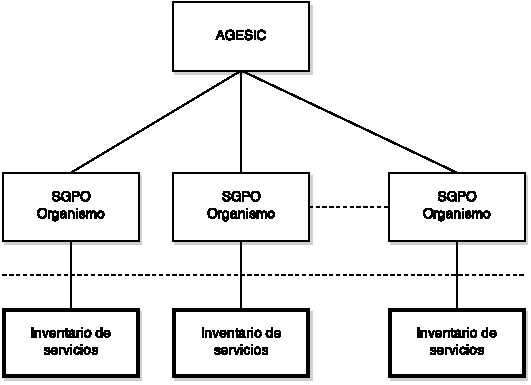
\includegraphics[width=\linewidth]{modelo_jurisdiccion_sgpo_propuesta}
      \caption{Modelo de jurisdicción de SGPO propuesto para la PDI}
      \label{Figura:ModeloJurisdiccionSGPOPropuesta}
    \end{figure}

    Para la adpción del modelo de jurisdicción se tienen en cuenta dos condiciones dadas en la realidad actual: (a) la influencia de AGESIC sobre los procesos de análisis, definición e implementación de servicios se encuentra limitada a aspectos de opción tecnológica, ya que las etapas iniciales del proceso ocurren en cada organismo por separado; y (b) la división de caracter político de los organismos coincide con las del tipo de información, asegurando que dos organismos no se encuentren desarrollando servicios tales que ofrezcan información repetida o que se solapen en el tipo de acción que realizan. Esta última da un claro indicio de separación de dominios, en donde cada organismo proveedor es un conjunto de servicios relacionados entre sí por una misma área de negocios. Este escenario permite la aplicación de un modelo de jurisdicción basado en SGPO dedicadas a cada dominio, funcionando en forma federada con una SGPO central gestionada por AGESIC.

    Este modelo se ajusta a la realidad actual de los organismos proveedores aplicando su propia gobernanza a su dominio de servicios, a la vez que le otorga a AGESIC la responsabilidad de establecer aspectos a todos los organismos desde la SGPO central. Es posible relativizar el ajuste a este modelo por parte de los organismos, dado que su autonomía les permite aplicar sus propias subdivisiones administrativas (SGPO por debajo de la del organismo, ciclos de vida de servicios distintos, entre otros); en esta propuesta se mantiene una visión de caja negra con respecto a los procesos administrativos en cada organismo, como se puede apreciar en la figura \ref{Figura:ModeloJurisdiccionSGPOPropuesta}. La gobernanza general aplicada desde la SGPO central se limitará a las actividades sobre las que tiene influencia AGESIC hoy en día: aspectos técnicos de publicación, de seguridad, procedimientos, entre otros. Todas aquellas decisiones que influyan sobre procesos internos a una SGPO independiente, no podrán ser tomadas por la SGPO central.

    La aplicación y comunicación de este modelo a los organismos les permitirá mantener a estos sus estructuras administrativas y de gestión actuales, y le dará visión a AGESIC sobre la estructura jerárquica de aplicación de la gobernanza.

  \subsection{Ciclo de vida de servicios}
    \label{Solucion:Gobernanza:CicloDeVida}

    \begin{figure}[h]
      \centering
      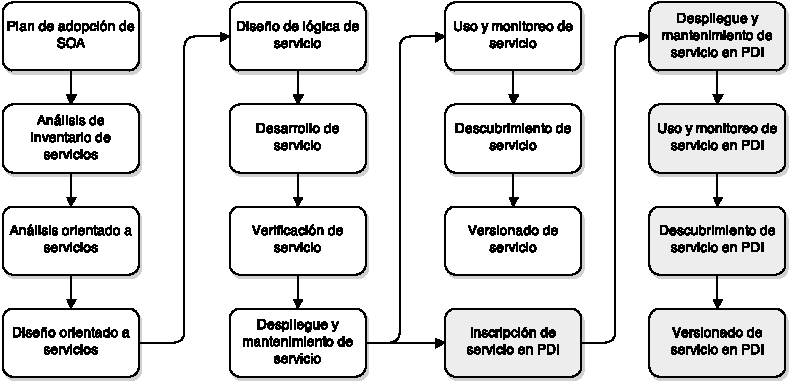
\includegraphics[width=\linewidth]{ciclo_de_vida_propuesta}
      \caption{Ciclo de vida de proyecto y servicios propuesto}
      \label{Figura:CicloDeVidaPropuesta}
    \end{figure}

    Este proceso es una adaptación del original tomado de \cite{Erl:2011:SGG:1983453}, a la cual se le agregan las etapas correspondientes a los procesos administrativos y técnicos. En la figura \ref{Figura:CicloDeVidaPropuesta} se presenta la secuencia propuesta para la publicación, monitoreo y versionado de servicios en la PDI gobernada por AGESIC, desde el inicio de su concepción en los organismos, pasando por su publicación en la infraestructura propia hasta llegar al subproceso de publicación en la plataforma. Las etapas contrastadas (de color más oscuro) son las gobernadas por AGESIC y comienzan a partir de la solicitud de publicación de un servicio. Cada servicio transcurre un proceso similar al mostrado en la figura, previo al punto de inscripción, y luego cumple con las etapas establecidas en el modelo propuesto.

    La independencia en la gobernanza de servicios de cada organismo (ya establecida en el modelo de jurisdicción propuesto en la sección \ref{Solucion:Gobernanza:ModeloJurisdiccion}), flexibiliza el ciclo de vida anterior a la inscripción de un servicio, pudiendo un organismo establecer su propio proceso antes de establecer un vínculo con la PDI. Si bien AGESIC establece normas técnicas de compatibilidad para la publicación, no se proponen restricciones a los procesos internos, siguiendo de la mano el modelo de jurisdicción.

    Esta independencia de procesos va de la mano con la realidad actual y el alcance de la gobernanza ejercida desde AGESIC, por lo que la propuesta resulta estar adaptada a las condiciones.

  \subsection{Gobernanza del ciclo de vida en AGESIC}
    \label{Solucion:Gobernanza:CicloDeVidaAGESIC}

    Ante la necesidad de proveer un nuevo servicio a través de la PDI, el organismo deberá contactar con AGESIC para hacer que el servicio se encuentre dentro de la plataforma y sea accesible por otros organismos. El proceso se describe en la figura \ref{Figura:ProcesoPublicacionPDI}.

    \begin{figure}[h]
      \centering
      % Pendiente
      \caption{Diagrama BPMN del proceso de publicación en la PDI}
      \label{Figura:ProcesoPublicacionPDI}
    \end{figure}

    \begin{enumerate}
      \item Inscripción de servicio
      \item Despliegue y mantenimiento de servicio
      \item Uso y monitoreo de servicio
      \item Descubrimiento de servicio
      \item Versionado de servicio
    \end{enumerate}

    \subsection{Inscripción de servicio}
      \label{Solucion:Gobernanza:CicloDeVidaAGESIC:Inscripcion}

      Un organismo proveedor de servicios que desea publicar su servicio deberá ponerse en contacto con AGESIC para dar inicio al proceso. Este comenzará rellenando un formulario vía web en una página alojada bajo el dominio de AGESIC\footnote{agesic.gub.uy} en el cual el personal a cargo de iniciar el trámite deberá detallar datos sobre el servicio a publicar, incluyendo características técnicas, responsables administrativos, ejemplos de uso, entre otros detallados en la figura \ref{Figura:TablaDatosInscripcion}. Este formulario será validado automáticamente verificando la completitud de los datos requeridos, a la vez que enviará una confirmación de recepción a la o las direcciones de correo electrónico especificadas con una copia de los datos ingresados en los campos y un código único de expediente o \emph{ticket} para la realización del seguimiento. La generación de este código es responsabilidad del sistema de gestión de la inscripción de servicios, el cual permitirá al personal administrativo de AGESIC la actualización del estado de los expedientes, de forma de permitir la realización del seguimiento del proceso por parte de los responsables en la parte proveedora.

      \begin{figure}[h]
        \centering
        % Pendiente
        \caption{Tabla de campos requeridos en el formulario de inscripción de un servicio}
        \label{Figura:TablaDatosInscripcion}
      \end{figure}

      Los expedientes deberán transitar por cuatro estados básicos establecidos: \emph{Iniciado}, \emph{Procesando}, \emph{Confirmado}, \emph{Completado}. Estos abarcan estados generales, pero se podrán identificar nuevos a medida que el proceso se optimice y así se crea necesario. Es posible diseñar el sistema de inscripción via web de forma que se integre a una aplicación de gestión de expedientes existente que así lo permita, adoptando los estados provistos de fábrica.

      El proceso de gestión de la inscripción debe seguir los pasos habituales de la realidad actual. Se destacan las negociaciones necesarias para establecer los criterios en el documento de acuerdo de nivel de servicios (\emph{SLA}), cuyo contenido está influenciado en gran medida por los datos técnicos aportados en el formulario de inscripción. El documento SLA debe establecer los acuerdos de nivel de servicio desde el proveedor en dirección hacia la PDI de forma tal que sea posible generar nuevos SLA entre AGESIC, el proveedor y los potenciales consumidores.

      La culminación de este proceso en forma exitosa da comienzo a la etapa de despliegue, abordada en la sección \ref{Solucion:Gobernanza:CicloDeVidaAGESIC:Despliegue}.

    \subsubsection{Despliegue y mantenimiento}
      \label{Solucion:Gobernanza:CicloDeVidaAGESIC:Despliegue}

      En esta etapa se lleva a cabo la configuración del acceso al servicio por parte de los consumidores a través de la PDI. Se asume completada la etapa de implantación en la plataforma del proveedor. En este caso, el objetivo es configurar una comunicación entre la PDI y el servicio desplegado del lado del organismo, de modo que los clientes de dicho servicio establezcan la comunicación con el lado del proveedor a través de la PDI de forma transparente. Para lograr esta comunicación se utilizará una tecnología que permita crear \emph{proxies} en la PDI, preconfigurados para redirigir el tráfico hacia la infraestructura del proveedor como se muestra en la figura \ref{Figura:ComunicacionProxyClienteProveedor}. Ejemplos de este tipo de tecnología son los \emph{Enterprise Service Bus (ESB)} de proveedores conocidos como JBoss\footnote{\url{https://www.jboss.org/jbossesb/}} o IBM\footnote{\url{http://www.ibm.com/software/products/en/wsesb/}}. Los procedimientos en cuanto a configuraciones de seguridad y acceso están fuera del alcance de esta propuesta.

      \begin{figure}[h]
        \centering
        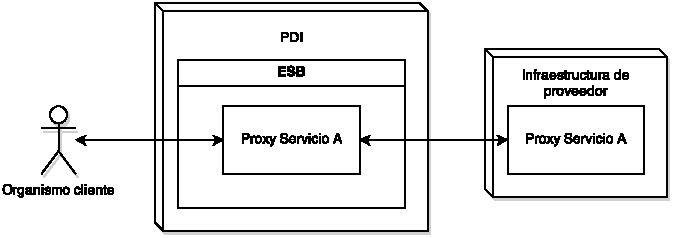
\includegraphics[width=\linewidth]{cliente_pdi_proveedor}
        \caption{Patrón «Proxy» aplicado a la comunicación entre cliente y proveedor}
        \label{Figura:ComunicacionProxyClienteProveedor}
      \end{figure}

      El rol de \emph{desarrollador} participa en las actividades llevadas a cabo en esta etapa, recibiendo la especificación del servicio para realizar las configuraciones pertinentes en la infraestructura de software de la PDI. Dicha especificación es obtenida a partir del proceso descrito en la sección \ref{Solucion:Gobernanza:CicloDeVidaAGESIC:Inscripcion}.

      Al completarse el proceso de configuración, se entra en fase de verificación para asegurar el cumplimiento de los requisitos de funcionamiento del servicio, así como también de los de calidad establecidos en el acuerdo de nivel de servicio (siglas en Inglés, SLA) entre AGESIC y el proveedor. El rol de \emph{especialista en el aseguramiento de la calidad (QA, por sus siglas en inglés)} dirige los procesos de verificación llevados a cabo, es decir, todos aquellos que aseguren una correcta comunicación entre la infraestructura de la plataforma de interoperabilidad y la del organismo proveedor del servicio, así como también el correcto funcionamiento de los controles de seguridad y acceso. No se verifica el funcionamiento en cuanto a la lógica del servicio en cuestión sino únicamente una comunicación exitosa; este tipo de verificación se asumirá completada por parte del organismo proveedor al momento de realizar el despliegue.

      El mantenimiento es un trabajo conjunto entre desarrolladores y especialistas en QA. Este implica una verificación periódica de los sistemas que mantienen al servicio disponible a través de la PDI y especialmente, en cumplimiento con su SLA a través de las métricas establecidas en el modelo de calidad aplicado. AGESIC debe encargarse de las tareas de mantenimiento necesarias para mantener la comunicación entre la PDI y el servicio del ldo del proveedor funcionando como se espera. Estas tareas de mantenimiento pueden requerir en ocasiones, una baja temporaria del servicio, afectando así a la disponibilidad. Se debe tomar en cuenta para evitar mayores dificultades, los horarios de uso establecido por los consumidores para realizar dichas tareas fuera de los horarios «pico» de utilización. Independientemente de la franja horaria en la que se realicen las tareas de mantenimiento, se deberá dar notificación de aquellas que sean programadas, en forma electrónica e inmediatamente luego de ser agendadas. Se proponen dos vías simultáneas como base: un servicio de novedades de tipo «feed de noticias» o alimentador, y comunicación vía correo electrónico a las direcciones de contacto provistas por los clientes. Esto permite a cualquier usuario del sistema, acceder a información sobre el estado de mantenimiento de los servicios, y permite la notificación en caso de que no exista una conducta de verificación regular del estado.

      Una tercera vía a implementar puede ser tomada de \emph{Google Apps Status Dashboard}\footnote{\url{http://www.google.com/appsstatus}}. Esta consiste en un sistema que lista los servicios disponibles y establece un color para el estado reportado en el que se encuentran al momento de ingresar al sitio. Cuando suceden errores que son detectados, u ocurren tareas de mantenimiento programadas, estas son identificadas con el color apropiado en dicho sitio.

      \emph{En desarrollo}

    \subsubsection{Uso y monitoreo}
      Durante el uso y monitoreo de los servicios, AGESIC se encargará de recolectar los valores de las mediciones correspondientes para asegurar la calidad y buen funcionamiento del servicio, así como también servir de retroalimentación para las actividades de mantenimiento y cobro por acceso.

      Periódicamente se realizarán actividades de revisión de funcionamiento sobre los servicios para determinar la necesidad de realizar ajustes sobre la configuración del acceso, independientemente de las revisiones de vitalidad que se realicen bajo la gobernanza del propio organismo sobre la lógica del servicio.

      Para realizar estas revisiones se tomarán en cuenta atributos de calidad que tengan impacto sobre la carga del servicio. Por ejemplo, un servicio que esté experimentando «picos» de uso periódicamente, deberá someter su configuración a revisión por parte del equipo de analistas de AGESIC para determinar la necesidad y viabilidad de un aumento de recursos para el proxy intermediario.

      Para hacer posible la detección de estas situaciones, se contará con un sistema de monitoreo sobre los servicios, el cual estará configurado en base a un modelo de calidad (abordado en la sección \ref{Solucion:Calidad}). No se especifica en esta propuesta una forma de monitoreo particular; en base a la infraestructura existente, se sugiere la instalación de módulos de medición de atributos de calidad en la infraestructura de un Enterprise Service Bus (ESB).

      \emph{En desarrollo}

    \subsubsection{Descubrimiento}
      Siguiendo el principio de \emph{Service Discoverability} (una ponderación sobre qué tan sencillo es encontrar un servicio), será necesario hacer que los servicios dispongan de suficientes meta-datos que permitan a un potencial usuario, descubrirlo y reutilizarlo en sus procesos de negocio, de manera de no solicitar la creación de nuevos servicios que cubran en todo o en parte lo que servicios ya existentes.

      Para facilitar el descubrimiento se establece una serie de meta-datos básicos de los que todos los servicios deben disponer. Esta información será desplegada en un registro central (central registry), gobernado por AGESIC. Este registro será independiente de los posibles registros gobernados por cada organismo, ya que contendrá sus propios meta-datos predefinidos y almacenados al momento de la publicación/migración.

      El acceso a este registro será público a través de la Internet. El sitio web se hará disponible a través de un servidor web gestionado por AGESIC. Se aplicará un criterio de confidencialidad sobre los meta-datos “sensibles”, de forma de no hacerlos disponibles a través del catálogo público, de existir.
      Algunos servicios podrán requerir ser marcados como privados, y por tanto sólo descubribles a en forma interna y con acceso autorizado. Esto deberá someterse a evaluación por parte del proveedor del servicio, en caso de que así se indique en la solicitud de publicación.

      Personal en el rol de custodio de servicios se encargaran de revisar los datos de los servicios publicados para asegurar la completitud y veracidad de los mismos. Un mismo custodio podrá estar encargado de más de un inventario de servicios, de ser necesario; no se establecen restricciones al respecto.

      El registro no permitirá la gestión del acceso al servicio a través de la web, sino que se continuará con el procedimiento actual de gestión de la publicación a través de formularios. Se sugiere con énfasis la implementación de un sistema electrónico independiente para la gestión de la publicación y solicitud de implementación de servicios.

      Ante situaciones de descubrimiento de servicios que resulten en solicitudes de modificaciones, las mismas serán transmitidas al organismo proveedor responsable y se pondrá en contacto al solicitante con dicho proveedor para negociar los cambios, los cuales, podrían resultar en una posterior migración de versión, situación descrita en la próxima sección.

      Una buena etapa de descubrimiento de servicios, requiere de la participación en la etapa del diseño orientado a servicio. Sin embargo, como hemos visto, AGESIC no participa de dicha etapa, por lo que la definición o modificación de meta-datos de uno o más servicios, puede requerir de contactar a los diseñadores responsables de cada uno.

      En la sección \ref{Implementacion:CasoEstudio} introducimos una descripción de la implementación de un prototipo de registro central de servicios.

      \emph{En desarrollo}

    \subsubsection{Versionado y retiro}
      Una nueva versión de un servicio será gestionada a partir de la solicitud por parte del organismo responsable. El procedimiento para la solicitud será similar al de la publicación, con el rellenado de un formulario especificando información relevante al cambio de versión. Esta actividad puede requerir de interacción entre responsables para determinar el procedimiento a seguir en cuanto a la configuración de la PDI y los cambios que potencialmente será necesario realizar para mantener el funcionamiento.

      Se aplicará la técnica de versionado desarrollada en la sección A DEFINIR.

      El retiro definitivo de servicios deberá ser planificado y anunciado cuanto antes a los organismos dependientes, de forma de permitirles establecer un curso de acción. Esto puede resultar difícil si el organismo proveedor omite el anuncio a AGESIC sobre la pre-determinación del retiro. Lo ideal será considerado que un servicio se encuentre en estado «deprecated» por un periodo no menor a 90 días, y esto sea anunciado con igual anticipación a los organismos dependientes. Pasado el periodo, el servicio (Proxy) será dado de baja de la PDI, así como también las configuraciones de seguridad y control de acceso establecidas para el mismo.

      Para determinar las dependencias, se utilizará un registro de consumidores de cada servicio, disponible desde el momento de cada suscripción.

      \emph{En desarrollo}
